\subsection{A deblending test}
\label{sec:deblending_test}

TODO: here, I look at results on a small $8 \times 8$ image in one band. I see how well we are able to deblend the image. 

Preliminary results are in Figure~\ref{fig:deblending_test}. 

I display the log-odds, $\log q(N = 2)  - \log q(N = 1)$, under our sleep-trained variational posterior. 

I compare against the true posterior, computed by gridding the sample space: we took a grid of $100\times 100$ locations and $100$ fluxes (for two stars, this had to be squared, for a total of $100^6$ samples ... it took awhile). 

Interestingly, the true posterior is biased towards two stars, even when the two stars are perfectly overlapping.

This actually makes sense. When two stars are perfectly overlapping (source separation = 0), the likelihood conditional on one bright star vs. the likelihood conditional on two stars each with half the brightness of the one star will be exactly the same. The prior (Poisson mean = 1) slightly encourages one star over two, but the flux distribution (which encourages dimmer stars) implicitly encourages two stars. In this example, these two prior terms seem to balance out. We see that when the separation is zero, the log-odds is about zero. 

Unfortunately, our variational posterior doesn't have the same behavior. The neural net just doesn't seem good enough to detect that there should be two stars? Also, the network seems very confident -- the log odds jump quickly from -5 (super confident of 1 star) to to 0.4 to 1 (super confident of two stars). 

\begin{figure}[!h]
    \centering
    \begin{subfigure}[t]{\textwidth}
    \centering
    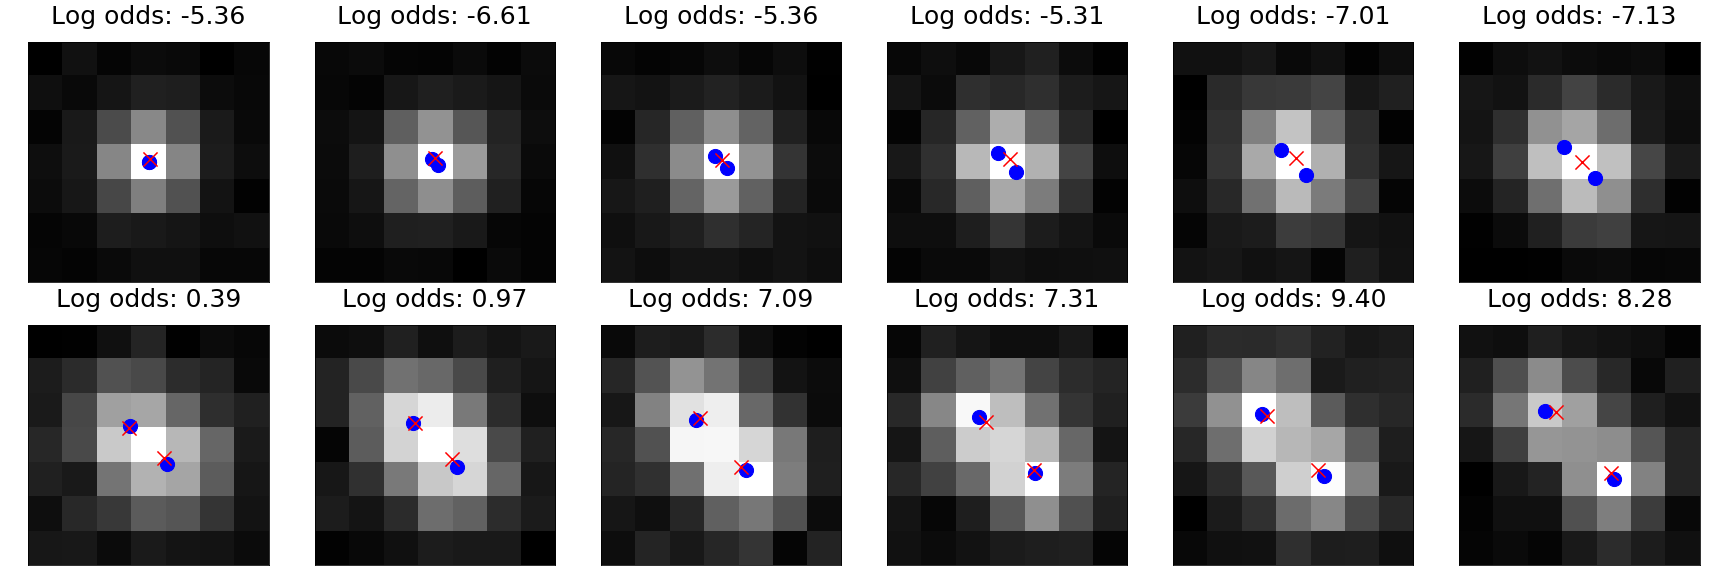
\includegraphics[width=\textwidth]{figures/deblending_ex.png}
    \end{subfigure}
    \begin{subfigure}[t]{\textwidth}
    \centering
    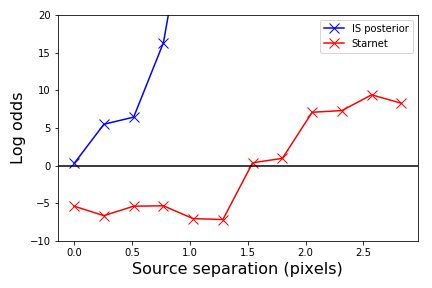
\includegraphics[width=0.5\textwidth]{figures/deblending_is_compare.png}
    \end{subfigure}
    \vspace{-3em}
    \caption{(Top) Detections as source separation increases. Red are MAP detections, blue are true locations. Log odds displayed are probability of two stars over probability of one star (Bottom) Comparison of log odds from the variational posterior and from the true posterior; the latter is computed by importance sampling. }
    \label{fig:deblending_test}
\end{figure}


In the final draft, I would also like have a more wide-ranging deblending test, similar to Figure 5 in~\cite{Feder_2019}, where we look at how well we deblend stars as fluxes and colors vary. 
